\usetikzlibrary{arrows, decorations.pathmorphing, calc, decorations.markings, intersections}
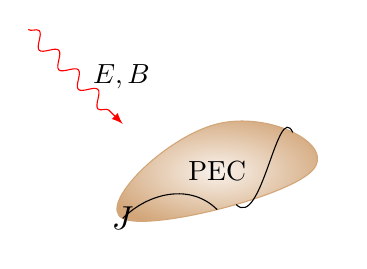
\begin{tikzpicture}[
  scale=1.2,
  photon/.style={decorate,decoration={snake,post length=1mm}},
  >=latex
]
  \node (p1) at (0, 0) {};
  \node (p2) at (1, 1) {};
  \node (p3) at (2, 0.5) {};
  \shadedraw[name path=mold, inner color=brown!10, outer color=brown!70, draw=brown!70]
    plot [smooth cycle,tension=1] coordinates {(p1) (p2) (p3)};

  \draw[->,red, photon] (-1, 2) -- node[above, right, xshift=0.1cm, black] {$\vb{E}, \vb{B}$} (0, 1);

  \node[] at (1, 0.5) {PEC};
  \path[name path=v1] (1,0) -- (1, 1);
  \path[name path=v2] (1.2,0) -- (1.2, 1);

  %\draw ($(p2)$) arc (-180:0:1mm);
  \draw [name intersections={of=v1 and mold}] (0, 0) to[out=45,in=135] (intersection-1);
  \draw [name intersections={of=v2 and mold}] (intersection-1) to[out=-45,in=115] (1.8, 0.91) node [midway] {$\vb{J}$};

\end{tikzpicture}
